% ============================================================
%  PriceIQ --- System Design Document
%  BTech Final Year Project, 2025-2026
% ============================================================
\documentclass[12pt,a4paper]{report}

\usepackage[top=1in,bottom=1in,left=1.2in,right=1in]{geometry}
\usepackage[utf8]{inputenc}
\usepackage[T1]{fontenc}
\usepackage{booktabs}
\usepackage{longtable}
\usepackage{array}
\usepackage{tabularx}
\usepackage{multirow}
\usepackage[hidelinks]{hyperref}
\usepackage{xcolor}
\usepackage{enumitem}
\usepackage{fancyhdr}
\usepackage{parskip}
\usepackage{setspace}
\usepackage{mdframed}
\usepackage{tikz}

\usetikzlibrary{positioning, arrows.meta, shapes.geometric, calc, fit, backgrounds}

\definecolor{priblue}{RGB}{0,82,165}
\definecolor{lightblue}{RGB}{210,230,255}
\definecolor{lightgreen}{RGB}{210,240,215}
\definecolor{lightyellow}{RGB}{255,250,205}
\definecolor{lightorange}{RGB}{255,235,210}
\definecolor{lightred}{RGB}{255,220,220}
\definecolor{lightgray}{RGB}{245,245,245}
\definecolor{darkgray}{RGB}{80,80,80}

\setlength{\headheight}{14pt}
\pagestyle{fancy}
\fancyhf{}
\fancyhead[L]{\small\textit{PriceIQ --- System Design Document v1.0}}
\fancyhead[R]{\small\textit{BTech Final Year Project 2025--2026}}
\fancyfoot[C]{\thepage}
\renewcommand{\headrulewidth}{0.4pt}

\setlength{\parskip}{6pt}
\setlength{\parindent}{0pt}
\onehalfspacing

\newcolumntype{L}[1]{>{\raggedright\arraybackslash}p{#1}}
\newcolumntype{C}[1]{>{\centering\arraybackslash}p{#1}}

\newmdenv[linecolor=priblue,backgroundcolor=lightblue!40,
          linewidth=1pt,skipabove=6pt,skipbelow=6pt]{notebox}

\begin{document}

% --- TITLE PAGE ---------------------------------------------------------------
\begin{titlepage}
  \centering
  \vspace*{1.8cm}
  {\Huge\bfseries\color{priblue} PriceIQ\par}
  \vspace{0.4cm}
  {\large AI-Powered Electronics Price Comparison for Indian Consumers\par}
  \vspace{1.4cm}
  \rule{0.85\linewidth}{1.5pt}\\[0.5cm]
  {\LARGE\bfseries System Design Document\par}
  \vspace{0.3cm}
  {\large Document Version 1.0\par}
  \rule{0.85\linewidth}{1.5pt}
  \vspace{1.8cm}

  \begin{tabular}{@{}ll@{}}
    \textbf{Project Type:}    & BTech Final Year Project \\[4pt]
    \textbf{Department:}      & Computer Science and Engineering \\[4pt]
    \textbf{Academic Year:}   & 2025--2026 \\[4pt]
    \textbf{Prepared By:}     & Adrij Bhadra \\[4pt]
    \textbf{Date:}            & April 2026 \\[4pt]
    \textbf{Document Status:} & Final \\
  \end{tabular}

  \vfill
  {\small Covers: Client-Server Architecture, ER Diagram, Data Flow Diagrams,\\
  Component Design, API Design, and Database Schema.}
\end{titlepage}

\tableofcontents
\newpage

% --- CHAPTER 1: INTRODUCTION --------------------------------------------------
\chapter{Introduction}

\section{Purpose}
This System Design Document (SDD) describes the architectural decisions,
component structures, data models, and data-flow characteristics of
\textbf{PriceIQ}. It complements the Software Requirements Specification and
provides the technical blueprint used during implementation.

\section{Scope}
The document covers the following design artefacts:
\begin{itemize}[noitemsep]
  \item Client-Server architecture and technology stack
  \item Entity-Relationship (ER) diagram for the database schema
  \item Data Flow Diagrams (DFD) at Context, Level-1, and Level-2
  \item Component-level design of the scraper subsystem
  \item REST API endpoint design
  \item Database schema with constraints
\end{itemize}

\section{Design Goals}
\begin{enumerate}[noitemsep]
  \item \textbf{Accuracy} --- The product matching engine must reject
        accessories, wrong storage variants, and wrong model tiers before
        any data is stored.
  \item \textbf{Modularity} --- Each scraper is an independent module; the
        scoring engine is shared via a pure-function interface.
  \item \textbf{Graceful Degradation} --- A failed scraper must not prevent
        results from the other scrapers from being returned.
  \item \textbf{Simplicity} --- Next.js API routes co-locate server logic with
        the UI framework, minimising operational overhead for a single-developer
        project.
\end{enumerate}

% --- CHAPTER 2: CLIENT-SERVER ARCHITECTURE ------------------------------------
\chapter{Client-Server Architecture}

\section{Overview}
PriceIQ follows a \textbf{three-tier client-server architecture}:

\begin{enumerate}[noitemsep]
  \item \textbf{Presentation Tier} --- React 19 components rendered server-side
        (SSR) by Next.js 16 and delivered to the user's browser.
  \item \textbf{Application Tier} --- Next.js API routes act as the backend,
        orchestrating scraping, database operations, and AI inference.
  \item \textbf{Data Tier} --- PostgreSQL 16 database managed by Prisma 7 ORM,
        running in a Docker container.
\end{enumerate}

External services (Groq API, Amazon India, Flipkart, Vijay Sales) are consumed
by the Application Tier only; the browser never communicates with them directly.

\section{Architecture Diagram}

\begin{figure}[ht]
\centering
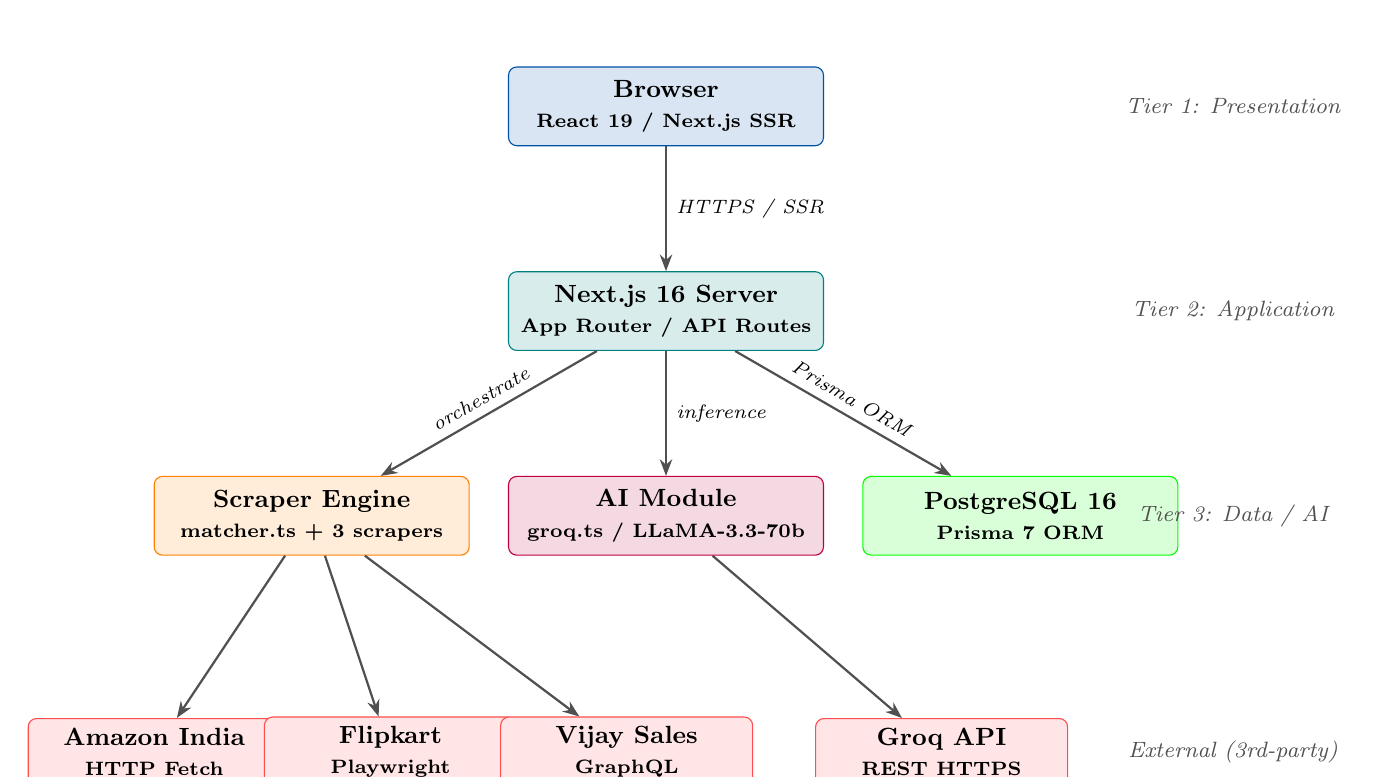
\begin{tikzpicture}[
  % align=center is required in all node styles to allow \\ line breaks
  layerbox/.style={rectangle, draw=#1, fill=#1!15, minimum width=4cm,
                   minimum height=1cm, align=center, rounded corners=3pt,
                   font=\small\bfseries},
  extbox/.style={rectangle, draw=red!70, fill=red!10, minimum width=3.2cm,
                 minimum height=0.85cm, align=center, font=\small\bfseries,
                 rounded corners=3pt},
  arr/.style={-{Stealth[length=6pt]}, thick, draw=darkgray},
  tierlabel/.style={font=\footnotesize\itshape, text=darkgray}
]

% Tier 1 - Browser
\node[layerbox=priblue] (browser) at (0, 0)
    {Browser\\{\scriptsize React 19 / Next.js SSR}};

% Tier 2 - Next.js Server
\node[layerbox=teal] (server) at (0, -2.6)
    {Next.js 16 Server\\{\scriptsize App Router / API Routes}};

% Tier 3 - Scraper / AI / DB
\node[layerbox=orange] (scrapers) at (-4.5, -5.2)
    {Scraper Engine\\{\scriptsize matcher.ts + 3 scrapers}};

\node[layerbox=purple] (ai) at (0, -5.2)
    {AI Module\\{\scriptsize groq.ts / LLaMA-3.3-70b}};

\node[layerbox=green] (db) at (4.5, -5.2)
    {PostgreSQL 16\\{\scriptsize Prisma 7 ORM}};

% External services
\node[extbox] (amazon)   at (-6.5, -8.2) {Amazon India\\{\scriptsize HTTP Fetch}};
\node[extbox] (flipkart) at (-3.5, -8.2) {Flipkart\\{\scriptsize Playwright}};
\node[extbox] (vs)       at (-0.5, -8.2) {Vijay Sales\\{\scriptsize GraphQL}};
\node[extbox] (groq)     at ( 3.5, -8.2) {Groq API\\{\scriptsize REST HTTPS}};

% Arrows
\draw[arr] (browser)  -- node[right, font=\scriptsize\itshape]{HTTPS / SSR} (server);
\draw[arr] (server)   -- node[above, font=\scriptsize\itshape, sloped]{orchestrate} (scrapers);
\draw[arr] (server)   -- node[right, font=\scriptsize\itshape]{inference}   (ai);
\draw[arr] (server)   -- node[above, font=\scriptsize\itshape, sloped]{Prisma ORM} (db);
\draw[arr] (scrapers) -- (amazon);
\draw[arr] (scrapers) -- (flipkart);
\draw[arr] (scrapers) -- (vs);
\draw[arr] (ai)       -- (groq);

% Tier labels on right
\node[tierlabel] at (7.2,  0)    {Tier 1: Presentation};
\node[tierlabel] at (7.2, -2.6)  {Tier 2: Application};
\node[tierlabel] at (7.2, -5.2)  {Tier 3: Data / AI};
\node[tierlabel] at (7.2, -8.2)  {External (3rd-party)};

\end{tikzpicture}
\caption{PriceIQ Three-Tier Client-Server Architecture}
\end{figure}

\section{Technology Stack}

\begin{longtable}{L{3.5cm} L{2.5cm} L{7cm}}
  \toprule
  \textbf{Layer} & \textbf{Technology} & \textbf{Rationale} \\
  \midrule
  \endhead
  Frontend Framework & Next.js 16.2.4 &
    App Router enables per-route server components and streaming SSR;
    eliminates a separate backend server. \\[3pt]
  UI Library & React 19.2.4 &
    Server and client components; concurrent rendering. \\[3pt]
  Styling & Tailwind CSS 4 &
    Utility-first; zero runtime CSS; dark-mode via \texttt{dark:} variants. \\[3pt]
  UI Components & Radix UI + shadcn/ui &
    Accessible, unstyled primitives; customised with Tailwind. \\[3pt]
  Charts & Recharts 3.8.1 &
    Declarative React charting; price history line chart and
    dashboard pie/bar charts. \\[3pt]
  ORM & Prisma 7.7.0 &
    Type-safe schema-first ORM; migrations via \texttt{db push}. \\[3pt]
  Database & PostgreSQL 16 &
    ACID-compliant relational DB; full-text search via \texttt{ilike}. \\[3pt]
  Browser Automation & Playwright 1.59.1 &
    Chromium headless browser for Flipkart DOM scraping with stealth headers. \\[3pt]
  LLM Inference & Groq SDK 1.1.2 &
    Hardware-accelerated inference; LLaMA-3.3-70b at very low latency. \\[3pt]
  Containerisation & Docker + Compose &
    Reproducible environment; Postgres volume for persistent data. \\
  \bottomrule
\end{longtable}

\section{Request-Response Flow for Live Search}
The complete flow for a live search request is as follows:

\begin{enumerate}[noitemsep]
  \item User types a query in the browser and submits the search form.
  \item Browser sends GET to \texttt{/search?q=\{query\}}.
  \item Next.js server component queries the database. If results are found,
        they are rendered and returned (\textbf{cache hit path}).
  \item If no results exist, the \texttt{LiveSearchTrigger} client component
        is rendered.
  \item The client component fires POST to \texttt{/api/search/live}.
  \item The API route calls \texttt{liveSearch(query)}.
  \item Vijay Sales (GraphQL) and Amazon (HTTP) scrapers execute in parallel
        via \texttt{Promise.allSettled}; Flipkart (Playwright) runs after.
  \item Each scraper passes candidate titles through \texttt{scoreCandidate()}
        and returns the best-accepted \texttt{NormalizedProduct}.
  \item Accepted products are upserted into the database; price history is
        recorded.
  \item \texttt{analyzeProduct()} is called to produce AI analysis via Groq.
  \item The API returns the new \texttt{productId}; client redirects to
        \texttt{/product/\{id\}}.
  \item The product page renders server-side with current listings and AI analysis.
\end{enumerate}

% --- CHAPTER 3: ER DIAGRAM ----------------------------------------------------
\chapter{Entity-Relationship Diagram}

\section{Database Schema Overview}
The PriceIQ database consists of five entities. All IDs are auto-generated
integers (Prisma default serial). All monetary values are stored as
\texttt{Float} in INR.

\section{ER Diagram}

\begin{figure}[ht]
\centering
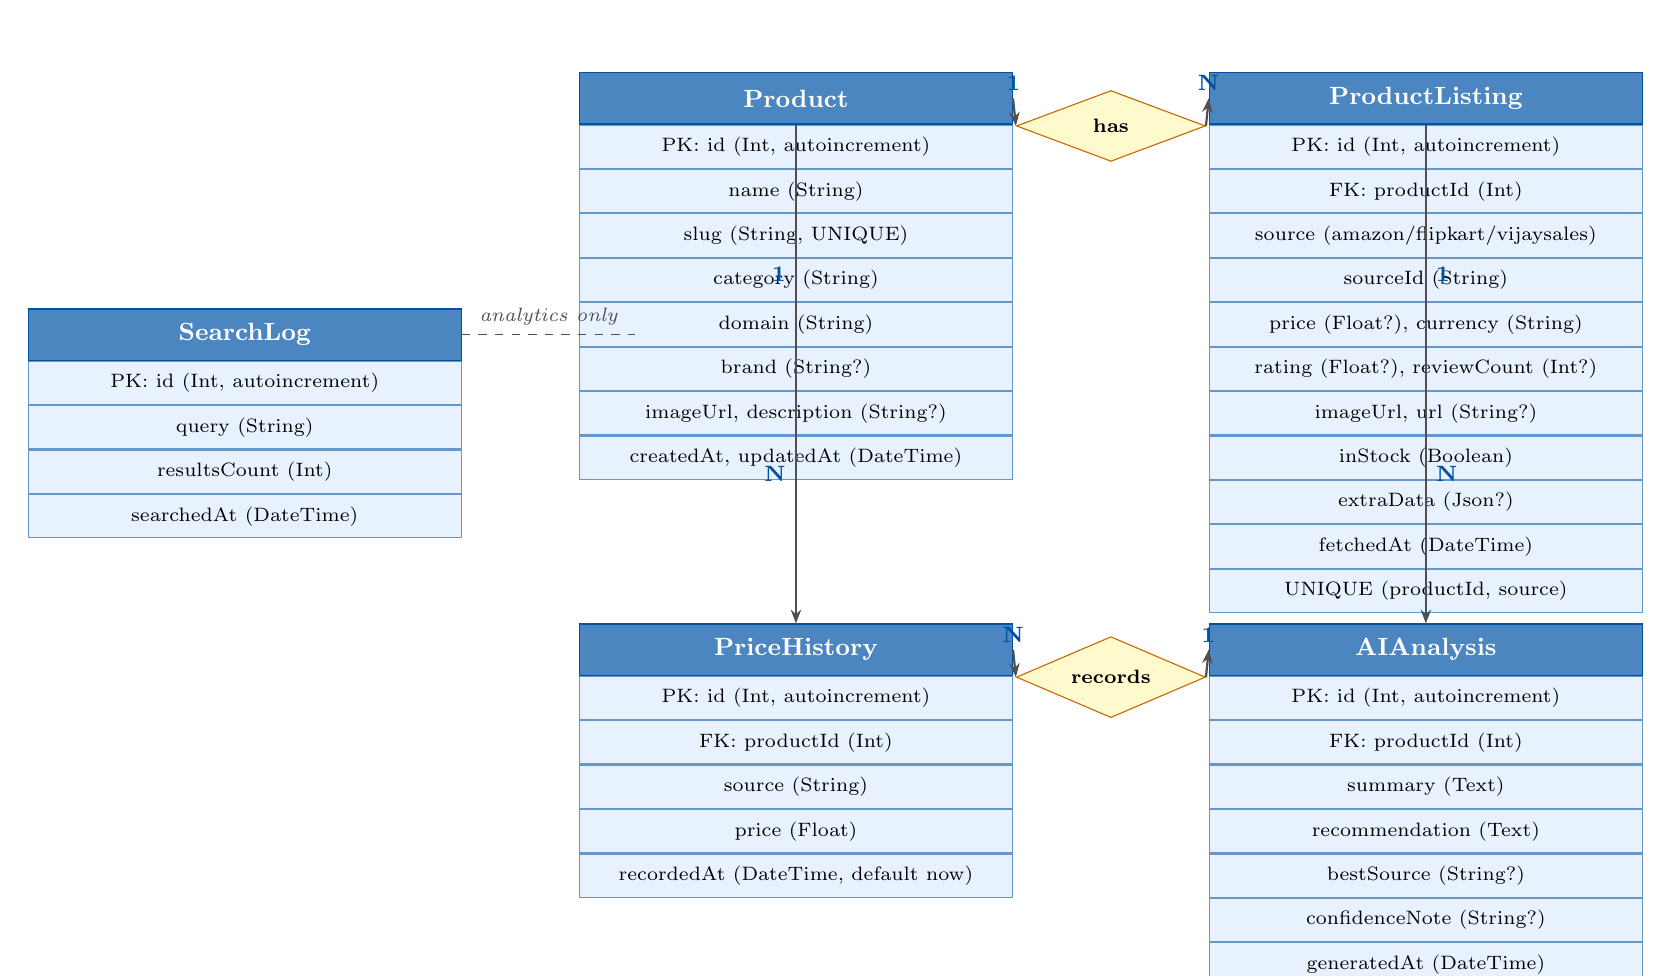
\begin{tikzpicture}[
  entityhdr/.style={rectangle, draw=priblue, fill=priblue!70,
                    minimum width=5.5cm, minimum height=0.65cm,
                    align=center, font=\small\bfseries\color{white}},
  entitybody/.style={rectangle, draw=priblue!60, fill=lightblue!50,
                     minimum width=5.5cm, minimum height=0.55cm,
                     align=left, font=\scriptsize, inner xsep=4pt},
  relhdr/.style={diamond, draw=orange!80!black, fill=lightyellow,
                 minimum width=2.4cm, minimum height=0.9cm,
                 align=center, font=\scriptsize\bfseries, aspect=2},
  arr/.style={-{Stealth[length=5pt]}, thick, draw=darkgray},
  card/.style={font=\footnotesize\bfseries, text=priblue}
]

% === Product entity (top-left) ===============================================
\node[entityhdr]                         (PE)  at (0,    0)    {Product};
\node[entitybody, below=0pt of PE]       (P1)  {PK: id (Int, autoincrement)};
\node[entitybody, below=0pt of P1]       (P2)  {name (String)};
\node[entitybody, below=0pt of P2]       (P3)  {slug (String, UNIQUE)};
\node[entitybody, below=0pt of P3]       (P4)  {category (String)};
\node[entitybody, below=0pt of P4]       (P5)  {domain (String)};
\node[entitybody, below=0pt of P5]       (P6)  {brand (String?)};
\node[entitybody, below=0pt of P6]       (P7)  {imageUrl, description (String?)};
\node[entitybody, below=0pt of P7]       (P8)  {createdAt, updatedAt (DateTime)};

% === ProductListing (top-right) ==============================================
\node[entityhdr]                         (LE)  at (8,    0)    {ProductListing};
\node[entitybody, below=0pt of LE]       (L1)  {PK: id (Int, autoincrement)};
\node[entitybody, below=0pt of L1]       (L2)  {FK: productId (Int)};
\node[entitybody, below=0pt of L2]       (L3)  {source (amazon/flipkart/vijaysales)};
\node[entitybody, below=0pt of L3]       (L4)  {sourceId (String)};
\node[entitybody, below=0pt of L4]       (L5)  {price (Float?), currency (String)};
\node[entitybody, below=0pt of L5]       (L6)  {rating (Float?), reviewCount (Int?)};
\node[entitybody, below=0pt of L6]       (L7)  {imageUrl, url (String?)};
\node[entitybody, below=0pt of L7]       (L8)  {inStock (Boolean)};
\node[entitybody, below=0pt of L8]       (L9)  {extraData (Json?)};
\node[entitybody, below=0pt of L9]       (L10) {fetchedAt (DateTime)};
\node[entitybody, below=0pt of L10]      (L11) {UNIQUE (productId, source)};

% === PriceHistory (bottom-left) ==============================================
\node[entityhdr]                         (HE)  at (0,   -7)    {PriceHistory};
\node[entitybody, below=0pt of HE]       (H1)  {PK: id (Int, autoincrement)};
\node[entitybody, below=0pt of H1]       (H2)  {FK: productId (Int)};
\node[entitybody, below=0pt of H2]       (H3)  {source (String)};
\node[entitybody, below=0pt of H3]       (H4)  {price (Float)};
\node[entitybody, below=0pt of H4]       (H5)  {recordedAt (DateTime, default now)};

% === AIAnalysis (bottom-right) ===============================================
\node[entityhdr]                         (AE)  at (8,   -7)    {AIAnalysis};
\node[entitybody, below=0pt of AE]       (A1)  {PK: id (Int, autoincrement)};
\node[entitybody, below=0pt of A1]       (A2)  {FK: productId (Int)};
\node[entitybody, below=0pt of A2]       (A3)  {summary (Text)};
\node[entitybody, below=0pt of A3]       (A4)  {recommendation (Text)};
\node[entitybody, below=0pt of A4]       (A5)  {bestSource (String?)};
\node[entitybody, below=0pt of A5]       (A6)  {confidenceNote (String?)};
\node[entitybody, below=0pt of A6]       (A7)  {generatedAt (DateTime)};

% === SearchLog (far-left) ====================================================
\node[entityhdr]                         (SE)  at (-7,  -3)    {SearchLog};
\node[entitybody, below=0pt of SE]       (S1)  {PK: id (Int, autoincrement)};
\node[entitybody, below=0pt of S1]       (S2)  {query (String)};
\node[entitybody, below=0pt of S2]       (S3)  {resultsCount (Int)};
\node[entitybody, below=0pt of S3]       (S4)  {searchedAt (DateTime)};

% === Relationships ===========================================================
% Product 1:N ProductListing
\node[relhdr] (R1) at (4, -0.35) {has};
\draw[arr] (PE.east) -- node[card, above, pos=0.1]{1} (R1.west);
\draw[arr] (R1.east) -- node[card, above, pos=0.9]{N} (LE.west);

% Product 1:N PriceHistory
\node[relhdr] (R2) at (4, -7.35) {records};
\draw[arr] (HE.east) -- node[card, above, pos=0.1]{N} (R2.west);
\draw[arr] (R2.east) -- node[card, above, pos=0.9]{1} (AE.west);

% Product -- PriceHistory (vertical left side)
\draw[arr] (PE.south) -- node[card, left, pos=0.3]{1}
           node[card, left, pos=0.7]{N}    (HE.north);

% Product -- AIAnalysis (vertical right side, skip over to right)
\draw[arr] (LE.south) -- node[card, right, pos=0.3]{1}
           node[card, right, pos=0.7]{N}   (AE.north);

% SearchLog (standalone -- no FK to Product, it's analytics only)
\draw[dashed, darkgray] (SE.east) -- node[above, font=\scriptsize\itshape]{analytics only}
      ++(2.2,0);

\end{tikzpicture}
\caption{PriceIQ Entity-Relationship Diagram}
\end{figure}

\section{Entity Descriptions}

\subsection{Product}
The central entity of the system. Each row represents one canonical
electronics product identified by a unique, URL-safe slug
(e.g., \texttt{iphone-15-128gb}). One product may have listings from
one, two, or all three retail platforms.

\subsection{ProductListing}
Each row represents the real-time state of a product on a specific retail
platform. The composite unique key \texttt{(productId, source)} ensures that
a re-scrape updates the existing row rather than inserting a duplicate.
The \texttt{extraData} JSON column stores platform-specific attributes such
as Vijay Sales MRP.

\subsection{PriceHistory}
An append-only table that records every price observation. A new row is
created on every scrape event (both live and batch). This table is the data
source for the price-trend line chart on the product page.

\subsection{AIAnalysis}
Stores the structured LLM output. Multiple rows per product are allowed; the
application always reads the most recent row (sorted by
\texttt{generatedAt} descending). The 24-hour cache TTL is enforced at the
application layer, not the database.

\subsection{SearchLog}
A simple analytics log. Each user search appends one row. No personally
identifiable information is stored (no user IDs or IP addresses).

% --- CHAPTER 4: DATA FLOW DIAGRAMS --------------------------------------------
\chapter{Data Flow Diagrams}

\section{DFD Level 0 --- Context Diagram}
The context diagram shows PriceIQ as a single process and its data exchanges
with all external entities.

\begin{figure}[ht]
\centering
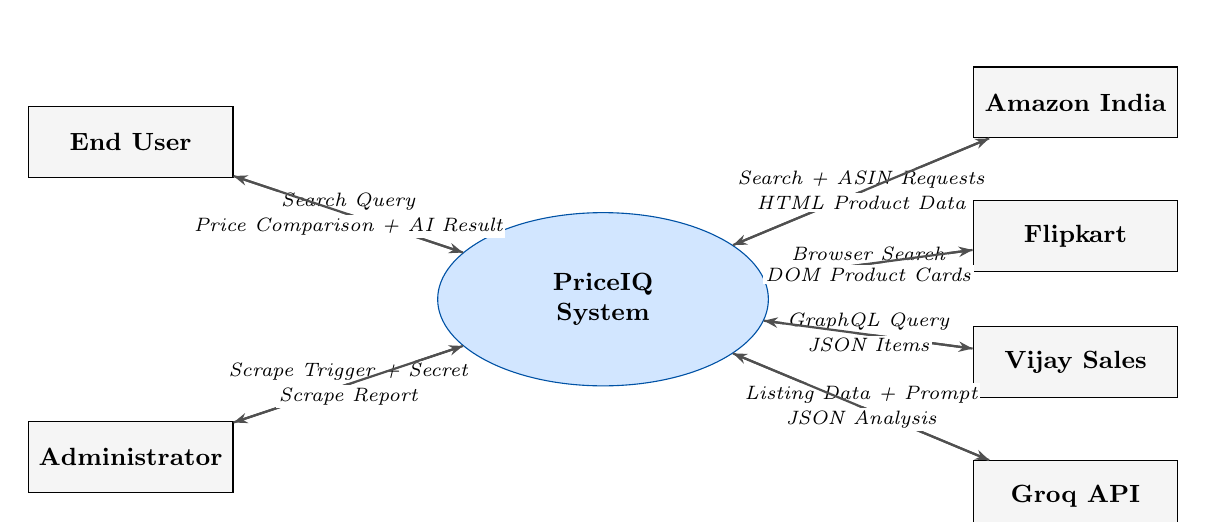
\begin{tikzpicture}[
  ext/.style={rectangle, draw=black, fill=lightgray,
              minimum width=2.6cm, minimum height=0.9cm,
              align=center, font=\small\bfseries},
  proc/.style={ellipse, draw=priblue, fill=lightblue,
               minimum width=4.2cm, minimum height=2.2cm,
               align=center, font=\small\bfseries},
  arr/.style={-{Stealth[length=5pt]}, thick, draw=darkgray},
  lbl/.style={font=\scriptsize\itshape, fill=white, inner sep=1pt}
]

\node[proc] (sys) at (0,0) {PriceIQ\\System};

\node[ext] (user)     at (-6,  2)   {End User};
\node[ext] (amazon)   at ( 6,  2.5) {Amazon India};
\node[ext] (flipkart) at ( 6,  0.8) {Flipkart};
\node[ext] (vs)       at ( 6, -0.8) {Vijay Sales};
\node[ext] (groq)     at ( 6, -2.5) {Groq API};
\node[ext] (admin)    at (-6, -2)   {Administrator};

\draw[arr] (user)  -- node[lbl,above]{Search Query} (sys);
\draw[arr] (sys)   -- node[lbl,below]{Price Comparison + AI Result} (user);

\draw[arr] (admin) -- node[lbl,above]{Scrape Trigger + Secret} (sys);
\draw[arr] (sys)   -- node[lbl,below]{Scrape Report} (admin);

\draw[arr] (sys)    -- node[lbl,above]{Search + ASIN Requests} (amazon);
\draw[arr] (amazon) -- node[lbl,below]{HTML Product Data} (sys);

\draw[arr] (sys)      -- node[lbl,above]{Browser Search} (flipkart);
\draw[arr] (flipkart) -- node[lbl,below]{DOM Product Cards} (sys);

\draw[arr] (sys) -- node[lbl,above]{GraphQL Query} (vs);
\draw[arr] (vs)  -- node[lbl,below]{JSON Items} (sys);

\draw[arr] (sys)  -- node[lbl,above]{Listing Data + Prompt} (groq);
\draw[arr] (groq) -- node[lbl,below]{JSON Analysis} (sys);

\end{tikzpicture}
\caption{DFD Level 0 --- PriceIQ Context Diagram}
\end{figure}

\newpage
\section{DFD Level 1 --- Main Processes}
The Level-1 diagram decomposes PriceIQ into five primary processes and two
data stores.

\begin{figure}[ht]
\centering
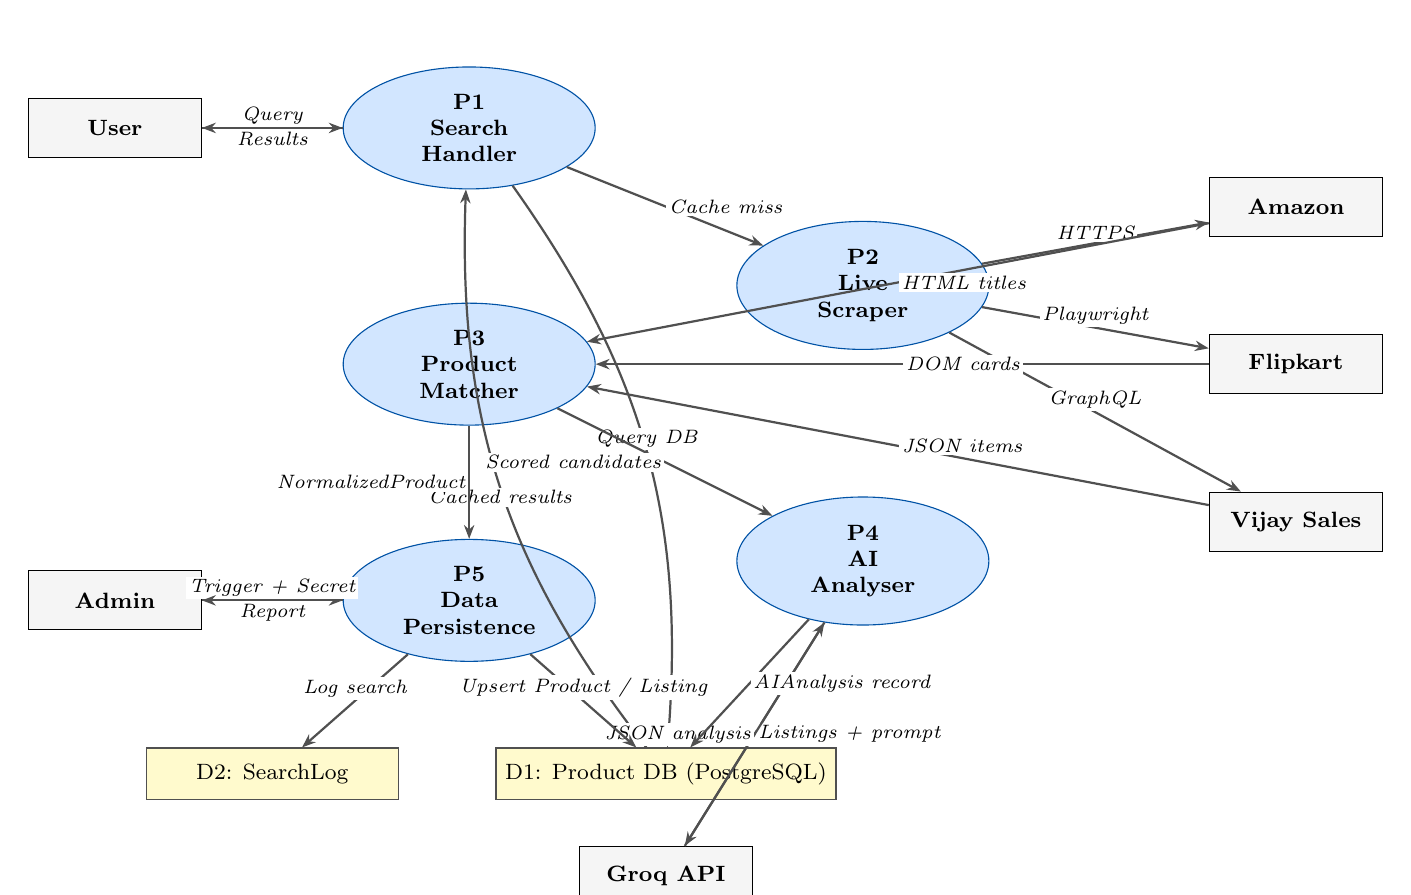
\begin{tikzpicture}[
  ext/.style={rectangle, draw=black, fill=lightgray,
              minimum width=2.2cm, minimum height=0.75cm,
              align=center, font=\footnotesize\bfseries},
  proc/.style={ellipse, draw=priblue, fill=lightblue,
               minimum width=3.2cm, minimum height=1.4cm,
               align=center, font=\footnotesize\bfseries},
  ds/.style={rectangle, draw=darkgray, fill=lightyellow,
             minimum width=3.2cm, minimum height=0.65cm,
             align=center, font=\footnotesize},
  arr/.style={-{Stealth[length=5pt]}, thick, draw=darkgray},
  lbl/.style={font=\scriptsize\itshape, fill=white, inner sep=1pt}
]

% External Entities
\node[ext] (user)     at (-7,  3)   {User};
\node[ext] (admin)    at (-7, -3)   {Admin};
\node[ext] (amazon)   at ( 8,  2)   {Amazon};
\node[ext] (flipkart) at ( 8,  0)   {Flipkart};
\node[ext] (vs)       at ( 8, -2)   {Vijay Sales};
\node[ext] (groq)     at ( 0, -6.5) {Groq API};

% Processes
\node[proc] (P1) at (-2.5,  3)    {P1\\Search\\Handler};
\node[proc] (P2) at ( 2.5,  1)    {P2\\Live\\Scraper};
\node[proc] (P3) at (-2.5,  0)    {P3\\Product\\Matcher};
\node[proc] (P4) at ( 2.5, -2.5)  {P4\\AI\\Analyser};
\node[proc] (P5) at (-2.5, -3)    {P5\\Data\\Persistence};

% Data Stores
\node[ds] (D1) at ( 0,  -5.2) {D1: Product DB (PostgreSQL)};
\node[ds] (D2) at (-5,  -5.2) {D2: SearchLog};

% User <-> P1
\draw[arr] (user) -- node[lbl,above]{Query}   (P1);
\draw[arr] (P1)   -- node[lbl,below]{Results} (user);

% Admin <-> P5
\draw[arr] (admin) -- node[lbl,above]{Trigger + Secret} (P5);
\draw[arr] (P5)    -- node[lbl,below]{Report} (admin);

% P1 -> P2 (miss) and P1 <-> D1 (hit)
\draw[arr] (P1) -- node[lbl,right]{Cache miss} (P2);
\draw[arr] (P1) to[bend left=20] node[lbl,above]{Query DB} (D1);
\draw[arr] (D1) to[bend left=20] node[lbl,below]{Cached results} (P1);

% P2 -> external scrapers
\draw[arr] (P2) -- node[lbl,above]{HTTPS}    (amazon);
\draw[arr] (P2) -- node[lbl,above]{Playwright} (flipkart);
\draw[arr] (P2) -- node[lbl,above]{GraphQL}  (vs);

% External -> P3
\draw[arr] (amazon)   -- node[lbl,right]{HTML titles}  (P3);
\draw[arr] (flipkart) -- node[lbl,right]{DOM cards}    (P3);
\draw[arr] (vs)       -- node[lbl,right]{JSON items}   (P3);

% P3 -> P4, P5
\draw[arr] (P3) -- node[lbl,left]{Scored candidates} (P4);
\draw[arr] (P3) -- node[lbl,left]{NormalizedProduct} (P5);

% P4 <-> Groq
\draw[arr] (P4)   -- node[lbl,right]{Listings + prompt} (groq);
\draw[arr] (groq) -- node[lbl,left]{JSON analysis}  (P4);

% P4 -> D1
\draw[arr] (P4) -- node[lbl,right]{AIAnalysis record} (D1);

% P5 -> D1, D2
\draw[arr] (P5) -- node[lbl,above]{Upsert Product / Listing} (D1);
\draw[arr] (P5) -- node[lbl,above]{Log search} (D2);

\end{tikzpicture}
\caption{DFD Level 1 --- Main Processes}
\end{figure}

\newpage
\section{DFD Level 2 --- P2 Live Scraper (Internal Flow)}
This diagram expands P2 (Live Scraper) to show the internal parallelism
and sequential flow between the three platform scrapers.

\begin{figure}[ht]
\centering
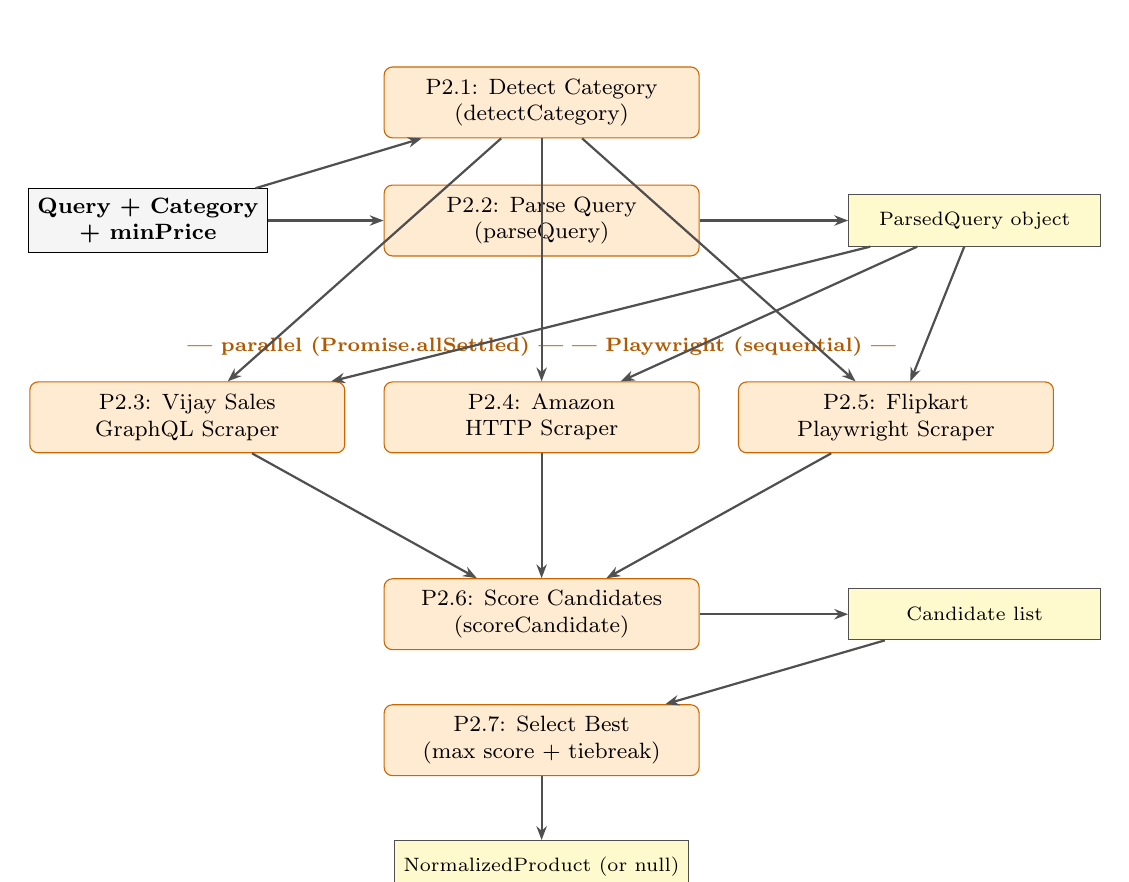
\begin{tikzpicture}[
  extnode/.style={rectangle, draw=black, fill=lightgray,
                  minimum width=2.6cm, minimum height=0.75cm,
                  align=center, font=\footnotesize\bfseries},
  subproc/.style={rectangle, draw=orange!80!black, fill=lightorange,
                  minimum width=4cm, minimum height=0.9cm,
                  align=center, font=\footnotesize, rounded corners=3pt},
  dsnode/.style={rectangle, draw=darkgray, fill=lightyellow,
                 minimum width=3.2cm, minimum height=0.65cm,
                 align=center, font=\scriptsize},
  arr/.style={-{Stealth[length=5pt]}, thick, draw=darkgray},
  lbl/.style={font=\scriptsize\itshape, fill=white, inner sep=1pt}
]

% Input
\node[extnode] (input) at (-5, 0)
    {Query + Category\\+ minPrice};

% Sub-processes
\node[subproc] (detectCat) at (0,  1.5)
    {P2.1: Detect Category\\(detectCategory)};
\node[subproc] (parseQ)    at (0,  0)
    {P2.2: Parse Query\\(parseQuery)};
\node[subproc] (vsS)   at (-4.5, -2.5)
    {P2.3: Vijay Sales\\GraphQL Scraper};
\node[subproc] (amzS)  at ( 0,   -2.5)
    {P2.4: Amazon\\HTTP Scraper};
\node[subproc] (fkS)   at ( 4.5, -2.5)
    {P2.5: Flipkart\\Playwright Scraper};
\node[subproc] (score) at ( 0,   -5)
    {P2.6: Score Candidates\\(scoreCandidate)};
\node[subproc] (selct) at ( 0,   -6.6)
    {P2.7: Select Best\\(max score + tiebreak)};

% Intermediate data stores
\node[dsnode] (parsed) at ( 5.5,  0)   {ParsedQuery object};
\node[dsnode] (cands)  at ( 5.5, -5)   {Candidate list};
\node[dsnode] (outn)   at ( 0,   -8.2) {NormalizedProduct (or null)};

% Parallel annotation (ASCII only)
\node[font=\scriptsize\bfseries, text=orange!70!black, align=center]
    at (0, -1.6)
    {--- parallel (Promise.allSettled) ---  --- Playwright (sequential) ---};

% Arrows
\draw[arr] (input) -- (detectCat);
\draw[arr] (input) -- (parseQ);
\draw[arr] (parseQ) -- (parsed);
\draw[arr] (parsed) -- (vsS);
\draw[arr] (parsed) -- (amzS);
\draw[arr] (parsed) -- (fkS);
\draw[arr] (detectCat) -- (vsS);
\draw[arr] (detectCat) -- (amzS);
\draw[arr] (detectCat) -- (fkS);
\draw[arr] (vsS)   -- (score);
\draw[arr] (amzS)  -- (score);
\draw[arr] (fkS)   -- (score);
\draw[arr] (score) -- (cands);
\draw[arr] (cands) -- (selct);
\draw[arr] (selct) -- (outn);

\end{tikzpicture}
\caption{DFD Level 2 --- P2 Live Scraper Internal Flow}
\end{figure}

\newpage
\section{DFD Level 2 --- P3 Product Matcher (Scoring Decision Tree)}
This diagram expands P3 (Product Matcher) to show the scoring decision tree
implemented in \texttt{matcher.ts}.

\begin{figure}[ht]
\centering
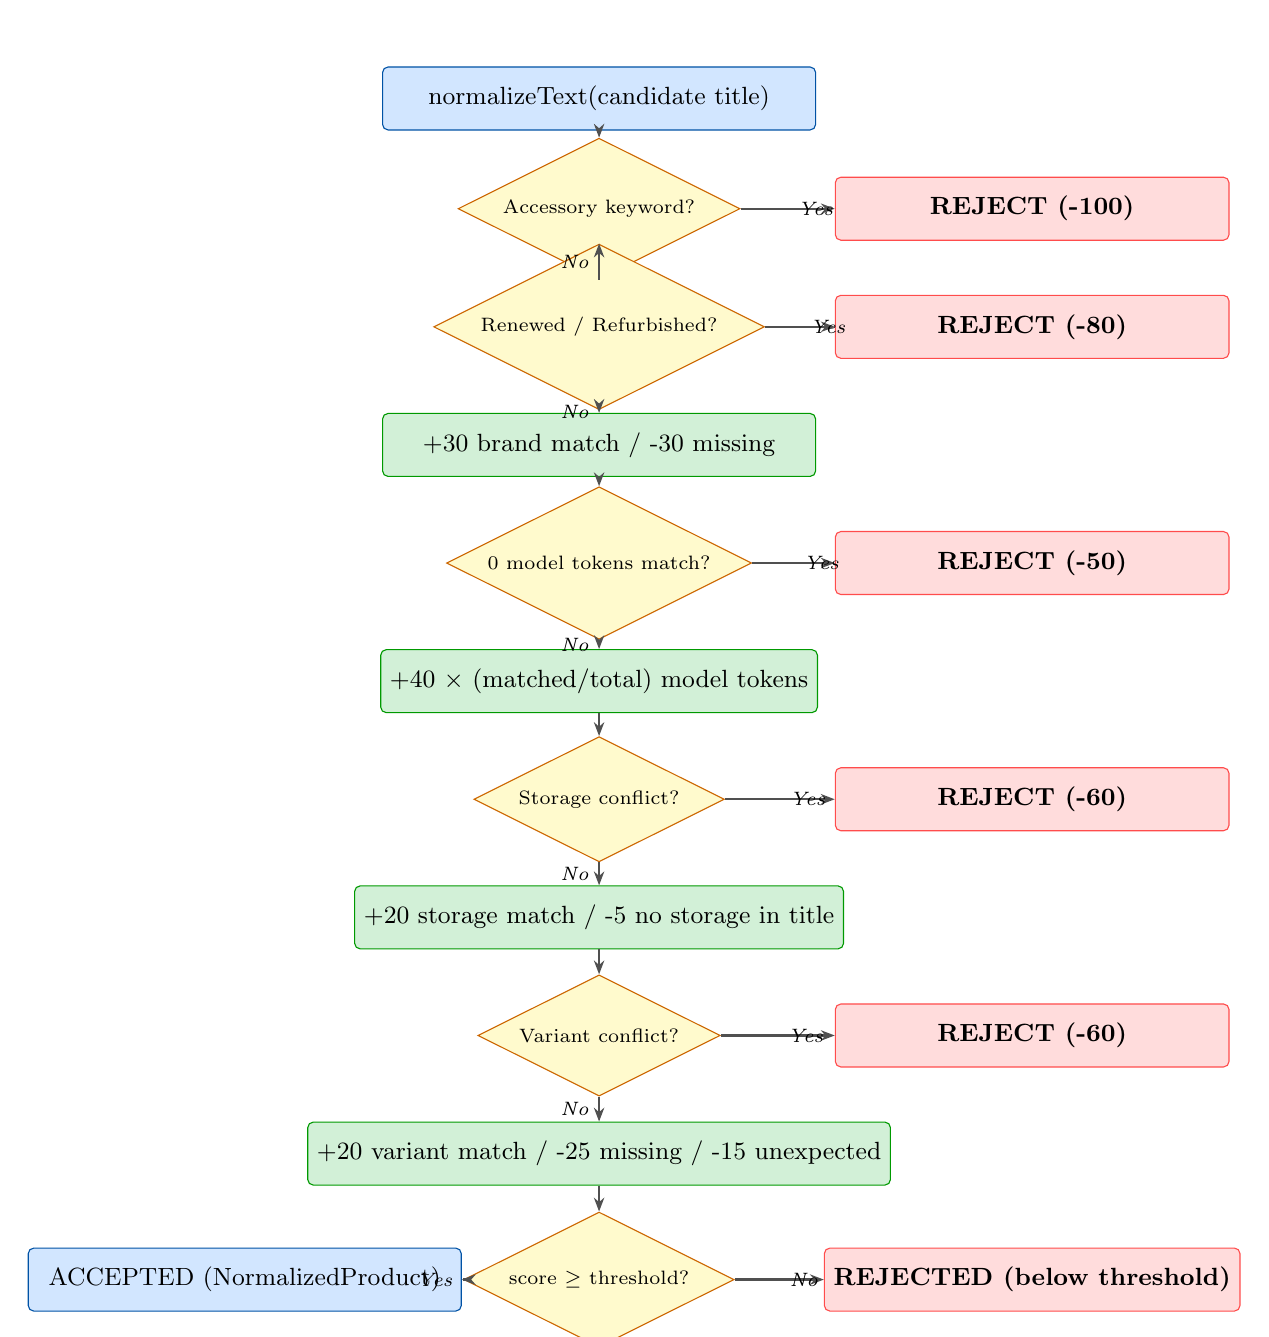
\begin{tikzpicture}[
  normbox/.style={rectangle, draw=priblue, fill=lightblue,
                  minimum width=5.5cm, minimum height=0.8cm,
                  align=center, font=\small, rounded corners=2pt},
  hardbox/.style={rectangle, draw=red!70, fill=lightred,
                  minimum width=5cm, minimum height=0.8cm,
                  align=center, font=\small\bfseries, rounded corners=2pt},
  softbox/.style={rectangle, draw=green!60!black, fill=lightgreen,
                  minimum width=5.5cm, minimum height=0.8cm,
                  align=center, font=\small, rounded corners=2pt},
  decbox/.style={diamond, draw=orange!80!black, fill=lightyellow,
                 minimum width=2cm, minimum height=0.9cm,
                 align=center, font=\scriptsize, aspect=2},
  arr/.style={-{Stealth[length=5pt]}, thick, draw=darkgray},
  lbl/.style={font=\scriptsize\itshape}
]

\node[normbox] (norm) at (0,    0)    {normalizeText(candidate title)};
\node[decbox]  (ac1)  at (0,  -1.4)  {Accessory keyword?};
\node[hardbox] (rj1)  at (5.5,-1.4)  {REJECT (-100)};
\node[decbox]  (ac2)  at (0,  -2.9)  {Renewed / Refurbished?};
\node[hardbox] (rj2)  at (5.5,-2.9)  {REJECT (-80)};
\node[softbox] (sb)   at (0,  -4.4)  {+30 brand match / -30 missing};
\node[decbox]  (ac3)  at (0,  -5.9)  {0 model tokens match?};
\node[hardbox] (rj3)  at (5.5,-5.9)  {REJECT (-50)};
\node[softbox] (sm)   at (0,  -7.4)  {+40 $\times$ (matched/total) model tokens};
\node[decbox]  (ac4)  at (0,  -8.9)  {Storage conflict?};
\node[hardbox] (rj4)  at (5.5,-8.9)  {REJECT (-60)};
\node[softbox] (ss)   at (0, -10.4)  {+20 storage match / -5 no storage in title};
\node[decbox]  (ac5)  at (0, -11.9)  {Variant conflict?};
\node[hardbox] (rj5)  at (5.5,-11.9) {REJECT (-60)};
\node[softbox] (sv)   at (0, -13.4)  {+20 variant match / -25 missing / -15 unexpected};
\node[decbox]  (thr)  at (0, -15)    {score $\geq$ threshold?};
\node[hardbox] (rj6)  at (5.5,-15)   {REJECTED (below threshold)};
\node[normbox] (ok)   at (-4.5,-15)  {ACCEPTED (NormalizedProduct)};

\draw[arr] (norm) -- (ac1);
\draw[arr] (ac1) -- node[lbl,right]{Yes} (rj1);
\draw[arr] (ac1) -- node[lbl,left] {No}  (ac2);
\draw[arr] (ac2) -- node[lbl,right]{Yes} (rj2);
\draw[arr] (ac2) -- node[lbl,left] {No}  (sb);
\draw[arr] (sb)  -- (ac3);
\draw[arr] (ac3) -- node[lbl,right]{Yes} (rj3);
\draw[arr] (ac3) -- node[lbl,left] {No}  (sm);
\draw[arr] (sm)  -- (ac4);
\draw[arr] (ac4) -- node[lbl,right]{Yes} (rj4);
\draw[arr] (ac4) -- node[lbl,left] {No}  (ss);
\draw[arr] (ss)  -- (ac5);
\draw[arr] (ac5) -- node[lbl,right]{Yes} (rj5);
\draw[arr] (ac5) -- node[lbl,left] {No}  (sv);
\draw[arr] (sv)  -- (thr);
\draw[arr] (thr) -- node[lbl,right]{No}  (rj6);
\draw[arr] (thr) -- node[lbl,left] {Yes} (ok);

\end{tikzpicture}
\caption{DFD Level 2 --- P3 Product Matcher Scoring Decision Tree}
\end{figure}

% --- CHAPTER 5: COMPONENT DESIGN ----------------------------------------------
\chapter{Component Design}

\section{Scraper Subsystem}
The scraper subsystem is located at \texttt{src/lib/scrapers/} and is composed
of the following modules:

\begin{longtable}{L{3cm} L{10cm}}
  \toprule
  \textbf{Module} & \textbf{Responsibility} \\
  \midrule
  \endhead
  \texttt{matcher.ts} &
    Pure-function scoring engine. Exports \texttt{normalizeText},
    \texttt{parseQuery}, and \texttt{scoreCandidate}. No side effects,
    no I/O. Can be unit-tested in isolation. \\[3pt]
  \texttt{products.ts} &
    Static catalogue of 4 products with per-source query strings and
    minimum price thresholds. Read-only data; no logic. \\[3pt]
  \texttt{vijaysales.ts} &
    Batch scraper: iterates PRODUCTS, calls the VS GraphQL endpoint, scores
    candidates, returns \texttt{NormalizedProduct[]}. \\[3pt]
  \texttt{amazon.ts} &
    Batch scraper: extracts ASINs from Amazon search HTML, fetches each
    product page, scores, returns best. \\[3pt]
  \texttt{flipkart.ts} &
    Batch scraper: one Playwright browser shared across all products;
    evaluates DOM to extract candidate cards; scoring in Node.js. \\[3pt]
  \texttt{live.ts} &
    On-demand scraper: \texttt{liveSearch(query)} orchestrates all three
    live scraper functions and returns aggregated results. \\[3pt]
  \texttt{index.ts} &
    Exports \texttt{runAllScrapers()} for the batch scrape API route. \\[3pt]
  \texttt{types.ts} &
    TypeScript interfaces (\texttt{NormalizedProduct}, \texttt{SourceName}).
    No runtime code. \\
  \bottomrule
\end{longtable}

\section{UI Component Hierarchy}

\begin{longtable}{L{4.5cm} L{8.5cm}}
  \toprule
  \textbf{Component} & \textbf{Responsibility} \\
  \midrule
  \endhead
  \texttt{layout.tsx} &
    Root layout: \texttt{ThemeProvider}, \texttt{Navbar},
    Sonner toast container. \\[3pt]
  \texttt{page.tsx} (home) &
    Marketing landing: \texttt{HeroSection}, \texttt{StatsBar},
    \texttt{FeaturesGrid}, \texttt{CategoryGrid}. \\[3pt]
  \texttt{search/page.tsx} &
    SSR results page: \texttt{SearchBar}, \texttt{SearchFilters},
    \texttt{ProductCard} grid, \texttt{LiveSearchTrigger} fallback. \\[3pt]
  \texttt{LiveSearchTrigger.tsx} &
    Client component: POST to \texttt{/api/search/live}, animated
    per-platform status, redirect on success. \\[3pt]
  \texttt{product/{[}id{]}/page.tsx} &
    SSR product detail: tabs for \texttt{PriceComparisonTable}
    and \texttt{AIRecommendation}. \\[3pt]
  \texttt{PriceComparisonTable.tsx} &
    Renders sorted listing cards with best-deal highlight
    and price-diff percentage. \\[3pt]
  \texttt{AIRecommendation.tsx} &
    Client component: lazy-fetches AI analysis; shows skeleton then result. \\[3pt]
  \texttt{PriceHistoryChart.tsx} &
    Recharts \texttt{LineChart} fetching
    \texttt{/api/price-history/[id]}. \\[3pt]
  \texttt{dashboard/page.tsx} &
    \texttt{KPICard}, \texttt{SourcePieChart}, \texttt{CategoryBarChart},
    \texttt{RecentSearches} table. \\
  \bottomrule
\end{longtable}

% --- CHAPTER 6: API DESIGN ----------------------------------------------------
\chapter{API Design}

All API routes are implemented as Next.js Route Handlers under
\texttt{src/app/api/}. JSON is the only data format. Error responses use
standard HTTP status codes with a JSON body \texttt{\{"error":"..."\}}.

\begin{longtable}{L{1.2cm} L{4.5cm} L{2.5cm} L{5cm}}
  \toprule
  \textbf{Method} & \textbf{Path} & \textbf{Auth?} & \textbf{Description} \\
  \midrule
  \endhead
  POST & \texttt{/api/search/live} & No &
    Run live scrape for a query. Body: \texttt{\{"query":"..."\}}.
    Returns \texttt{\{productId, aiAnalysis\}}. \\[3pt]
  GET & \texttt{/api/search} & No &
    Full-text product DB search. Params: \texttt{q}, \texttt{category},
    \texttt{source}, \texttt{sort}. Returns product array. \\[3pt]
  GET & \texttt{/api/search/suggestions} & No &
    Returns up to 5 product name suggestions matching \texttt{q}. \\[3pt]
  GET & \texttt{/api/products} & No &
    Paginated product list. Params: \texttt{page}, \texttt{limit}. \\[3pt]
  GET & \texttt{/api/products/[id]} & No &
    Single product with all listings. \\[3pt]
  GET & \texttt{/api/product/[id]} & No &
    Product detail including listings and latest AI analysis. \\[3pt]
  POST & \texttt{/api/product/[id]/refresh} & No &
    Trigger re-scrape for a specific product by ID. \\[3pt]
  POST & \texttt{/api/ai/analyze} & No &
    Generate or refresh AI analysis. Body: \texttt{\{productId\}}. \\[3pt]
  GET & \texttt{/api/price-history/[id]} & No &
    Full price history array for a product. \\[3pt]
  GET & \texttt{/api/dashboard} & No &
    Aggregated KPI statistics for the dashboard page. \\[3pt]
  POST & \texttt{/api/scrape} &
    Yes (\texttt{x-scrape-secret}) &
    Trigger full batch scrape. Returns \texttt{\{upserted: N\}}. \\
  \bottomrule
\end{longtable}

\section{Score Engine Public Interface}

\begin{longtable}{L{4.5cm} L{8.5cm}}
  \toprule
  \textbf{Function Signature} & \textbf{Description} \\
  \midrule
  \endhead
  \texttt{parseQuery(raw, category,}\\
  \texttt{minPrice) -> ParsedQuery} &
    Extracts structured intent from a raw search string: brand, model tokens,
    storageToken, variantToken. Passed to all scraper scoring calls. \\[3pt]
  \texttt{scoreCandidate(title, parsedQ)}\\
  \texttt{-> MatchResult} &
    Returns \texttt{\{score, accepted, reasons\}}.
    \texttt{accepted} is the gate for DB storage. \\[3pt]
  \texttt{normalizeText(text) -> string} &
    Lowercases, joins model codes (e.g.\ WH-1000XM5 to wh1000xm5),
    removes non-alphanumeric characters. \\
  \bottomrule
\end{longtable}

\chapter*{Revision History}
\begin{longtable}{C{1.5cm} C{2cm} L{4cm} L{5cm}}
  \toprule
  \textbf{Version} & \textbf{Date} & \textbf{Author} & \textbf{Changes} \\
  \midrule
  \endhead
  \bottomrule
  \endlastfoot
  1.0 & April 2026 & Adrij Bhadra &
    Initial release covering architecture, ER diagram, three-level DFDs,
    component design, API design, and database schema. \\
  \bottomrule
\end{longtable}

\end{document}
